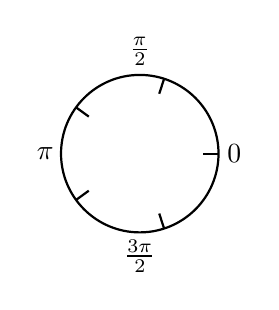
\begin{tikzpicture}
  % Draw the main circle (S^1)
\draw[thick] (0,0) circle(1);

% Parameters
\def\n{5}      % Number of truncation lines (Z5)
\def\r{1}      % Radius of the circle
\def\len{0.2}  % Length of the inward lines

% Draw the 5 truncation lines
\foreach \k in {0,...,4} {
  \draw[thick]
    ({\r*cos(360/\n*\k)}, {\r*sin(360/\n*\k)}) % start point on circle
    -- ({(\r-\len)*cos(360/\n*\k)}, {(\r-\len)*sin(360/\n*\k)}); % inward point
}

\node at (1.2, 0) {$0$};
\node at (0, 1.3) {$\frac{\pi}{2}$};
\node at (-1.2, 0) {$\pi$};
\node at (0, -1.3) {$\frac{3\pi}{2}$};

  
\end{tikzpicture}
